\documentclass[twoside,11pt]{report}

% Any additional packages needed should be included after jmlr2e.
% Note that jmlr2e.sty includes epsfig, amssymb, natbib and graphicx,
% and defines many common macros, such as 'proof' and 'example'.
%
% It also sets the bibliographystyle to plainnat; for more information on
% natbib citation styles, see the natbib documentation, a copy of which
% is archived at http://www.jmlr.org/format/natbib.pdf

\usepackage{jmlr2e}
% \usepackage[utf8]{inputenc}%
% \usepackage{tikz}
% \usepackage{cfr-lm}%
\usepackage[T1]{fontenc}%
\usepackage{physics}
\usepackage{amsmath}
% \usepackage{amssymb}
% \usepackage{graphicx}
% \usepackage[margin=3cm]{geometry}
% \usepackage{changepage}
\usepackage{fontspec}
\usepackage{minted}
\usepackage{tcolorbox}
\usepackage{lmodern}
\usepackage{xcolor}
\usepackage{lettrine}
% \usepackage{fontawesome}
\usemintedstyle{perldoc}
\usepackage{hyperref}
\hypersetup{colorlinks=false, pdfborder={0 0 0},  }
\usepackage{fancyhdr}
\usepackage{wrapfig}
\usepackage{adjustbox}
\usepackage{tikz}
\usepackage{listofitems} % for \readlist to create arrays



\newtcbox{\codebox}[1][black]{on line, arc=2pt,colback=#1!10!white,colframe=white, before upper={\rule[-3pt]{0pt}{10pt}},boxrule=1pt, boxsep=0pt,left=2pt,right=2pt,top=1pt,bottom=.5pt}
\newtcbox{\deloppg}[1][black]{on line, arc=2pt,colback=#1!10!white,colframe=white, before upper={\rule[-2pt]{0pt}{0pt}},boxrule=0pt, boxsep=0pt,left=.49\linewidth,right=.49\linewidth,top=4pt,bottom=3pt}


\newcommand\blfootnote[1]{ \begingroup \renewcommand\thefootnote{}\footnote{#1} \addtocounter{footnote}{-1} \endgroup }
% \definecolor{antwhite}{HTML}{323333}
\newcommand{\code}[3][]{\codebox{\mintinline[#1]{#2}{#3}}}



% \setmainfont{FreeSans}
% \setmainfont{SF Pro Display}
% \setmainfont{IBM Plex Sans}
% \setmainfont{TeX Gyre Heros}
% \setmainfont{Inter}
% \setmainfont{Iosevka Quasi}
% \setmainfont{DM Sans}

% \setmonofont{Iosevka Custom Extended}
% \setmonofont{JetBrainsMono Nerd Font}
\setmonofont[Scale=MatchLowercase]{DM Mono}





% Definitions of handy macros can go here

\newcommand{\dataset}{{\cal D}}
\newcommand{\fracpartial}[2]{\frac{\partial #1}{\partial  #2}}

% Heading arguments are {volume}{year}{pages}{submitted}{published}{author-full-names}

% \jmlrheading{1}{2000}{1-48}{4/00}{10/00}{https://github.com/bragewiseth/MachineLearningProjects}

% Short headings should be running head and authors last names

\ShortHeadings{\url{https://github.com/bragewiseth/MachineLearningProjects}}{\url{https://github.com/bragewiseth/MachineLearningProjects}}
\firstpageno{1}



\title{{\huge Project 1}}
\author{\name Brage W. \email bragewi@ifi.uio.no\\
       \name Felix C. H.  \email felixch@ifi.uio.no \\
       \name Eirik B. J. \email eiribja@ifi.uio.no}
\date{\today}											% Date
\makeatletter






% \date{\today}

\begin{document}

%%%%%%%%%%%%%%%%%%%%%%%%%%%%%%%%%%%%%%%%%%%%%%%%%%%%%%%%%%%%%%%%%%%%%%%%%%%%%%%%%%%%%%%%%

\begin{titlepage}
	\centering
    \vspace*{0.5 cm}
    \includegraphics[scale = 0.75]{uio.jpg}\\[1.0 cm]	% University Logo
    \textsc{\LARGE University of Oslo}\\[2.0 cm]	    % University Name
	\textsc{\Large FYS-STK3155}\\[0.5 cm]				% Course Code
	\rule{\linewidth}{0.2 mm} \\[0.4 cm]
	{ \huge \bfseries \@title}\\
	\rule{\linewidth}{0.2 mm} \\[1.5 cm]

	\begin{minipage}{0.4\textwidth}
		\begin{flushleft} \normalsize
            Brage Wiseth\\
            Felix Cameren Heyerdahl\\
            Eirik Bjørnson Jahr\\
			\end{flushleft}
			\end{minipage}~
			\begin{minipage}{0.4\textwidth}
			\begin{flushright} \normalsize
        \textsc{
          bragewi@ifi.uio.no\\
          felixch@ifi.uio.no\\
          eiribja@ifi.uio.no\\
        }
		\end{flushright}
        
	\end{minipage}\\[2 cm]
	\@date\\
    \vspace*{25mm}
    \urlstyle{rm}
    \textsc{\url{https://github.com/bragewiseth/MachineLearningProjects}}
	
	
    
    
    
    
	
\end{titlepage}
\nocite{*}
% \maketitle
\newpage
\tableofcontents
\newpage




\begin{abstract}%   <- trailing '%' for backward compatibility of .sty file
\lettrine{I}{}n this paper, we delve into the realm of machine learning model optimization and evaluation. 
Our study encompasses various regression techniques, including Ordinary Least Squares (OLS), Ridge, and 
Lasso regression, to analyze their effectiveness in handling simple and more complex datasets. Additionally, 
we employ bootstrap resampling and cross-validation methodologies to rigorously assess model performance 
and enhance generalization.
A significant portion of our investigation is dedicated to understanding the delicate balance between 
bias and variance. We explore how regularization methods like Ridge and Lasso impact bias-variance trade-offs, 
offering insights into the stability and predictive power of these models. Furthermore, we provide empirical 
evidence of the benefits of cross-validation and bootstrap techniques in mitigating overfitting and improving 
model robustness. We found that \{ ..results.. \}. Additionally we verify and compare our findings with well 
established theory and libraris such as SKLearn.
\end{abstract}
\begin{keywords}
    Linear Regression, Scaling, Bias \& Variance 
\end{keywords}









\section{Introduction}

Machine learning has emerged as a powerful tool in data analysis, providing the ability to uncover complex 
patterns and relationships in diverse datasets. But, at its core, machine learning is all about finding 
functions that capture the underlying structure of the data. The use of machine learning algorithms 
to approximate functions is the essence of this paper.\\

Our motivation for this research lies in the exploration of machine learning techniques to approximate 
the terrain on our planet, which can perhaps be described by such a function. Earth's terrain exhibits 
peaks and troughs, hills and valleys, much like some polynomial functions. Fortunately, we can employ 
standard linear regression techniques to approximate polynomials, but the terrain presents its own set 
of challenges. Firstly, the terrain's true underlying function may not be a polynomial at all, and its complexity may 
vary significantly from one location to another. Secondly, our landscape is teeming with small, intricate 
details. Some regions are characterized by flat and smooth surfaces, while others are marked by rough and 
uneven terrain. Focusing too much on these minute details can lead to model overfitting, making it crucial 
to strike a careful balance between model complexity and generalization.
In this context, regularization and resampling techniques, including Ridge and Lasso regression with bootstrap
and cross validation, have proven indispensable. By introducing regularization and resampling, we aim to find 
the sweet spot between bias and Variance. And getting the best predictions we can with our assumptions.\\
To embark on this exploration, we will begin with a simpler case: "Franke's function." which mimics our real terrain
data. This function 
serves as a foundational starting point, allowing us to assess our model's performance in a controlled 
environment before venturing into the complexity of real-world terrain data. Through this gradual progression, 
we provide ourselves wih a framework that can be applied to more complex and varied real-world terrain datasets.\\

\textbf{Data}: We begin by introducing the dataset used for our analysis, highlighting data collection and preprocessing procedures. 
Understanding the characteristics of the terrain data is fundamental to our modeling endeavor.\\
\textbf{Methods and Scaling}: Next, we delve into the methodology, encompassing the implementation of polynomial regression 
models and the application of regularization techniques such as Ridge and Lasso. Additionally, we will discuss the 
importance of proper scaling for model stability and convergence.\\
\textbf{Results}: In this section, we will present the outcomes of our experiments, showcasing the performance of different 
models and regularization techniques. Through empirical evidence, we aim to provide insights into the effectiveness of our approach.\\
\textbf{Bias-Variance Trade-off}: A significant portion of our study will revolve around the critical concept of bias and 
variance. We'll explore how regularization methods influence this trade-off and delve into the fine balance between 
model complexity and generalization.\\
\textbf{Conclusion}: Finally, we will summarize the key findings and their implications for terrain modeling with machine learning. 
Our conclusion will underscore the importance of regularization in achieving accurate representations of complex terrains and 
provide a perspective on future research directions.

\begin{center}
    \scriptsize code for generating all figures and data can be found at 
\href{https://github.com/bragewiseth/MachineLearningProjects/tree/main/project1/src}{\tt \textsc{/MachineLearningProjects/project1/src} }
\end{center}








\section{Data}
\label{sec:data}



\includegraphics[width=\linewidth]{nn.pdf}
\includegraphics[width=\linewidth]{bernoli.pdf}


\begin{tikzpicture}
    \draw[->] (0,0,0) -- (5,0,0) node[right] {$x$};
    \draw[->] (0,0,0) -- (0,5,0) node[above] {$y$};
    \draw[->] (0,0,0) -- (0,0,5) node[below left] {$z$};
\end{tikzpicture}

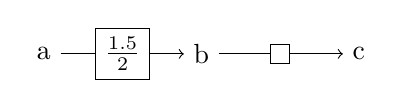
\begin{tikzpicture}
    \node (a) at (1,0) {a};
    \node (b) at (3,0) {b};
    \node (c) at (5,0) {c};
    \node[draw] (box1) at (2,0) {$\frac{1.5}{2}$};
    \node[draw] (box2) at (4,0) {};
    \draw[-] (a) -- (box1);
    \draw[->] (box1) -- (b);
    \draw[-] (b) -- (box2);
    \draw[->] (box2) -- (c);
\end{tikzpicture}




\begin{tikzpicture}
    \draw (0,0) .. controls (1,2) and (2,-1) .. (3,2);
\end{tikzpicture}



% The data we will be using consists of 100 points generated using the Franke function. The Franke function is a weighted sum of four exponentials given by
% \begin{align*}
%     f(x,y) &= \frac{3}{4}\exp\left(-\frac{(9x-2)^2}{4}-\frac{(9y-2)^2}{4}\right)\\
%     &+ \frac{3}{4}\exp\left(-\frac{(9x+1)^2}{49}-\frac{(9y+1)}{10}\right)\\
%     &+ \frac{1}{2}\exp\left(-\frac{(9x-7)^2}{4}-\frac{(9y-3)^2}{4}\right)\\
%     &- \frac{1}{5}\exp\left(-(9x-4)^2-(9y-7)^2\right)
% \end{align*}
% We will add some noise to the data to better simulate real world data. The data is generated by sampling $x$ and $y$ from a uniform distribution on the interval $[0,1]$. The noise is sampled from a normal distribution with mean 0 and standard deviation $\sigma = 0.1$.
% \begin{figure}[!h]
% \begin{minipage}[!t]{.48\linewidth}
%     \begin{center}
%         \includegraphics[width=1.1\textwidth]{../runsAndAdditions/trueFunction.png}
%         \caption{True Function}\label{fig:truefunction}
% \end{center}
% \end{minipage}
% \hspace{2mm}
% \begin{minipage}[!t]{.48\linewidth}
%     \begin{center}
%         \includegraphics[width=1.1\textwidth]{../runsAndAdditions/synthDataSide.png}
%         \caption{Our Synthetic Data}\label{fig:synthdataside}
%     \end{center}
% \end{minipage}
% \end{figure}
% \begin{figure}[!h]
% \begin{minipage}[!t]{.48\linewidth}
%     \begin{center}
%         \includegraphics[width=1.0\textwidth]{../runsAndAdditions/realdata3D.png}
%         \caption{True Function}\label{fig:realdata3D}
% \end{center}
% \end{minipage}
% \hspace{2mm}
% \begin{minipage}[!t]{.48\linewidth}
%     \begin{center}
%         \includegraphics[width=1.0\textwidth]{../runsAndAdditions/realdataMap.png}
%         \caption{Our Synthetic Data}\label{fig:realdataMap}
%     \end{center}
% \end{minipage}
% \end{figure}
% The noise is sampled from a normal distribution with mean 0 and standard deviation $\sigma = 0.1$.
% The data is generated by sampling x and y from a uniform distribution on the interval \[0, 1\].
% This synthetic data is divided into training and testing sets, with the testing set comprising twenty percent and the training set comprising eighty percent of the total data.
% In addition, we will incorporate genuine topographic data from a specific area of Norway. However, to reduce computational requirements when running the program, we've reduced the size of this real topographic dataset from 6.5 million points to 10,000 points.














\section{linear regression models }
\label{sec:models}






\subsection{Ordinary Least Squares (OLS)}
\label{sec:ols}


\subsection{Scaling}
\label{sec:scaling}









\section{Results and Discussion}
\label{sec:resultsdiscussion}



\subsection{Confidence Interval}
\label{sec:confidenceinterval}









\section{Bias \& Variance}
\label{sec:biasvariance}









\section{Conclusion}
\label{sec:conclusion}






















% \acks{}



% APPENDIX

%
%
\newpage
\appendix
\phantomsection%
\addcontentsline{toc}{section}{Appendix}
\section*{Appendix}
\label{app:appendix}




\phantomsection%
\addcontentsline{toc}{subsection}{Analytical Least Squares}
\subsection*{Derivation of The Optimal Parameters $\boldsymbol{\beta}$}
\label{app:OptimalBeta}







\phantomsection%
\addcontentsline{toc}{subsection}{SVD}
\subsection*{SVD}
\label{app:svd}





\phantomsection%
\addcontentsline{toc}{subsection}{Confidence Interval}
\subsection*{Math Behind the Confidence Interval, Section~\ref{sec:confidenceinterval}}
\label{app:confidenceinterval}




\vskip 0.2in
\bibliography{report}
% \bibliographystyle{apalike}
\bibliographystyle{plain}
\phantomsection%
\addcontentsline{toc}{section}{Bibliography}
\end{document}








